\subsubsection{State of the Art} 
I 2015 under Consumer Electronics Show (CES), viste tre firmaer hver en bil frem, som viser hvor langt de hver i ser er, i udviklingen af selv-kørende biler.\cite{CES}
\subsubsubsection{Audi A7}
\begin{figure}[h!]
	\centering
	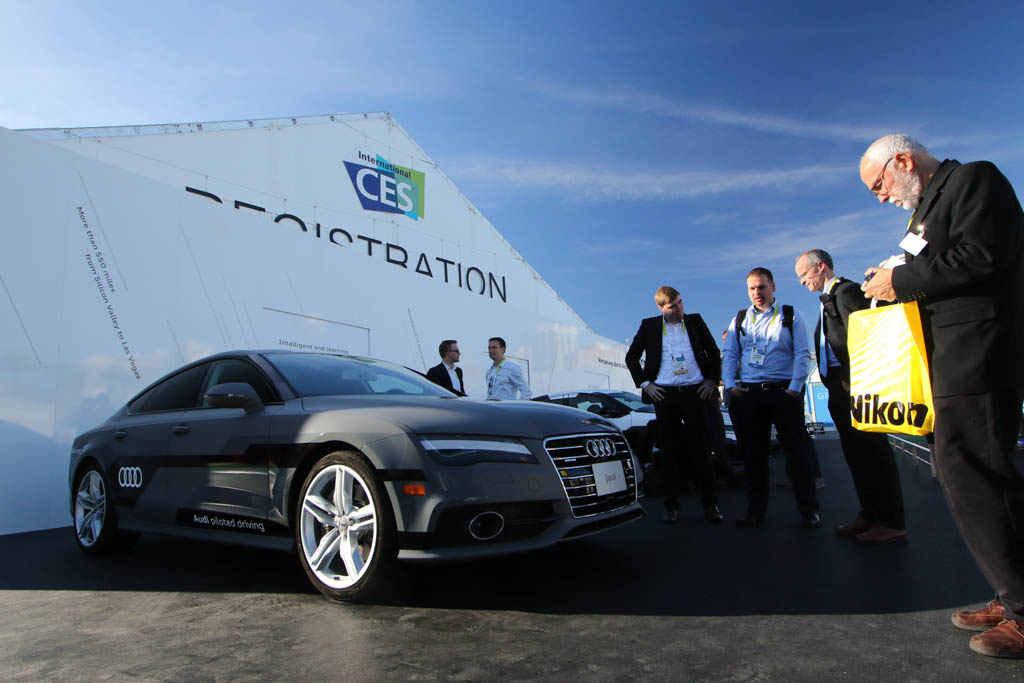
\includegraphics[width=0.8\textwidth]{images/150106_0345_ces.jpg}
	\captionsource{Audi A7 på 2015 CES}{\url{https://a248.e.akamai.net/f/574/7105/8d/www.extremetech.com/wp-content/uploads/2015/01/150106\_0345\_ces.jpg}}
	\label{fig:Audi_A7}
\end{figure}
Audi viste deres A7 frem, hvilken af de tre ligner mest en almindelig personbil (se figur \ref{fig:Audi_A7}), men den kan selv køre over lange distancer. Hvis den dog opdager mange mennesker i et område, typisk hvis den kører imod en by, vil den bede personen bag rattet om at overtage styrringen. Bilen havde inden konferencen kørt med nye trafikkanter og journalister fra Silicon Valley til Las Vegas, en distance på omkring 900km, næsten uden input fra føreren og dette selvom bilen kørte 110km/t. Bilen benytter sig af sensorer som allerede bliver fabrikeret, som også er i stand til præcist at se bilens omgivelser. Sensorene inkluderer adaptiv fartkontrol, overvågning over blinde vinkler, varsling hvis du er ved at køre af vejen og tre typer sensorer som allerede bliver brugt i diverse fartøjer i dag. Desuden kommer bilen også med andre sensorer så som laserscannere og kameraer, som gør bilen i stand til bedre at opdage objekter, både hvis objekterne er i bevægelse og hvis de er stillestående. Kameraerne, som optager i 3D, hjælper bilen med at holde styr på omkringværende trafik. Bilen er i stand til at køre på veje som ikke har høje bakker, hvor ingen biler pludseligt kører ind i din kørebane, eller en bil foran panikbremser.

\subsubsubsection{Mercedes-Benz F 015}
Denne bil blev lavet som et proof-of-concept, og vil ikke blive sat i produktion da udsynet for passagerne er alt for småt, men den indeholder teknologi og idéer som ikke er set før. F 015 har LED på hver side af forenden, som hjælper fodgængere med at se om det er sikkert for dem at gå ud foran bilen --- en slags alternativ til fodgængerfelter og trafiklys i dag. Disse LED'er følger fodgængerens mens han eller hun går forbi bilen, og viser dermed at bilen har øje med dem. Disse LED'er kan ses på bilen på figur \ref{fig:Mercedes-Benz_F_015}.
\begin{figure}[h!]
	\centering
	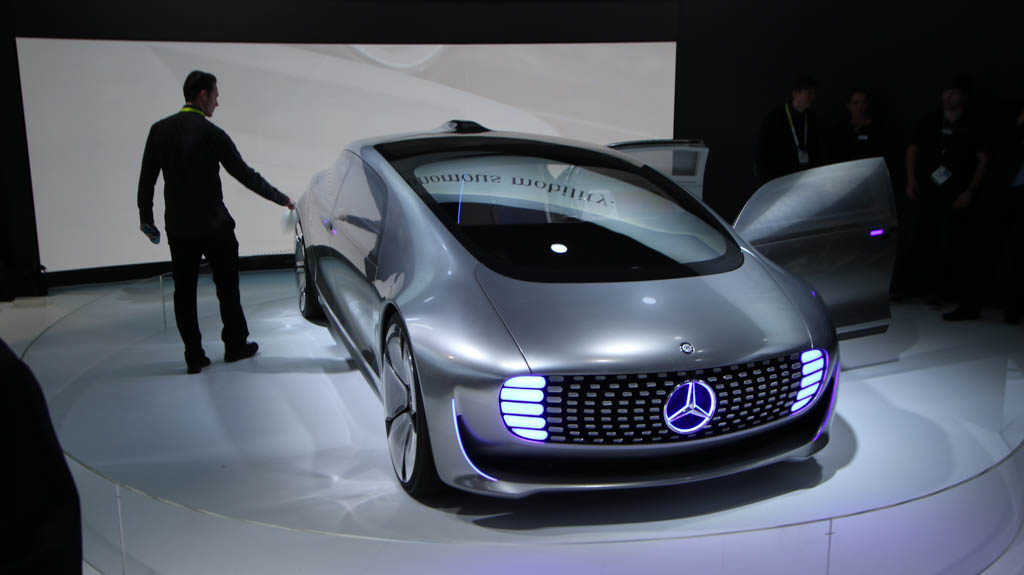
\includegraphics[width=0.8\textwidth]{images/150106_0422_ces.jpg}{}
	\captionsource{Mercedes-Benz konceptbilen F 015}{\url{https://a248.e.akamai.net/f/574/7105/8d/www.extremetech.com/wp-content/uploads/2015/01/150106\_0422\_ces.jpg}}
	\label{fig:Mercedes-Benz_F_015}
\end{figure}
\FloatBarrier
Fodgængere kan potentielt krydse vejen hvor de har lyst, hvis bilerne på vejen indikerer det er sikkert nok for dem. Forsæderne i bilen vender imod bagsæderne, hvilket gør alle folk i bilen, i stand til at holde øjekontakt under samtaler. Sæderne har også mulighed for at rotere horisontalt, så passagerne nemt kan stige ind og ud af bilen.
\subsubsubsection{BMW i3}
BMW tog en eksisterende bil og modificerede den indenfor et helt bestemt område; parkering. Bilen på figur \ref{fig:BMW_i3} er i stand til at parkere sig selv, og ikke ligesom vi i dag kender det, hvor bilen parallelparkerer. Med BMW i3 kan man køre hen til indgangen til en parkeringsplads, gå ud af bilen, og BMW i3 vil selv køre rundt på parkeringspladsen indtil den finder en fri plads. Herefter parkerer den selv, låser og slukker. Når man har brug for bilen igen, kan man inde i BMWs smartphone app til bilen tilkalde den, og så bare vente ved indgangen til parkeringspladsen, hvor bilen selv vil køre hen og samle dig op. Ikke kun skal bilen være i stand til at navigere rundt, den skal også være i stand til at undgå andre bilister, parkerede biler og ikke parkere på parkeringspladser prioriteret til handicappede.
\FloatBarrier
\begin{figure}[h!]
	\centering
	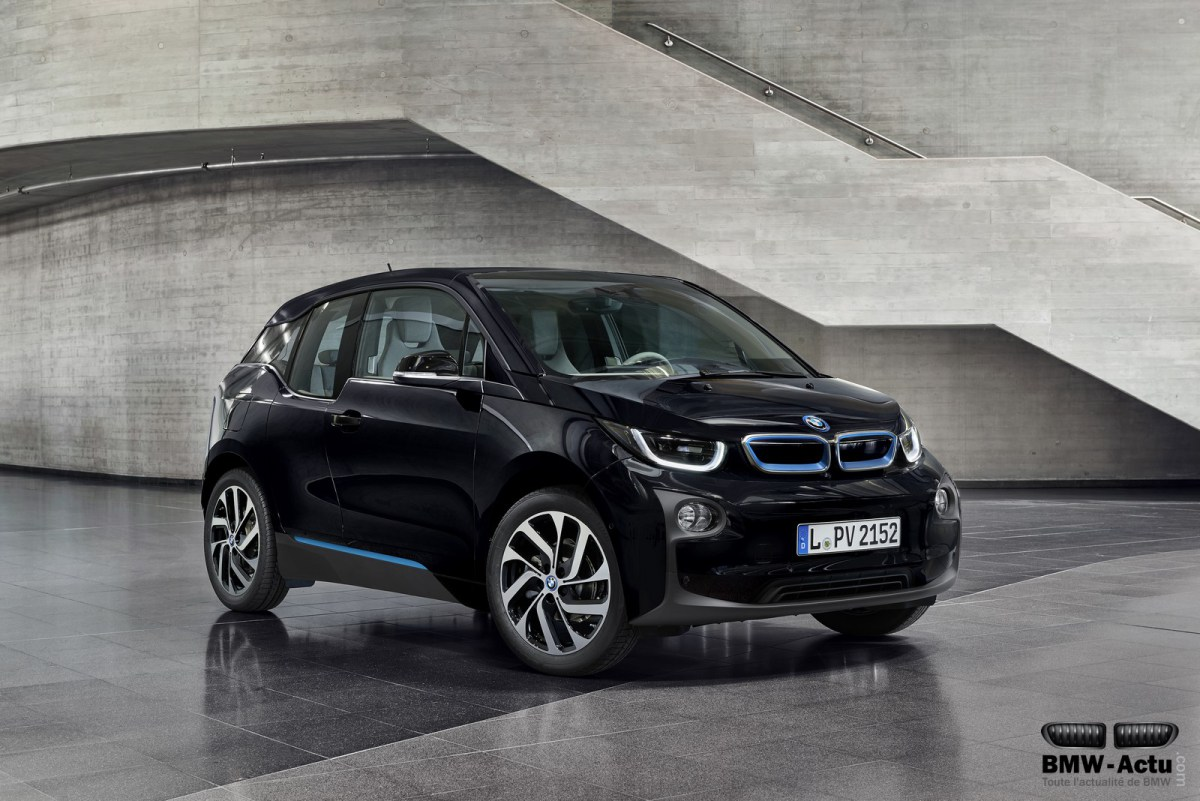
\includegraphics[width=0.8\textwidth]{images/bmw-i3-fluid-black-1.jpg}
	\captionsource{Den selv-parkerende BMW i3}{\url{https://bmwactu.files.wordpress.com/2015/09/bmw-i3-fluid-black-1.jpg}}
	\label{fig:BMW_i3}
\end{figure}
\FloatBarrier